\documentclass[11pt,a4paper]{article}
\usepackage{fontspec}
\setmainfont[Path=fonts/,FontIndex=7,BoldFont=AvenirNext.ttc,BoldFeatures={FontIndex=2},ItalicFont=AvenirNext.ttc,ItalicFeatures={FontIndex=4},BoldItalicFont=AvenirNext.ttc,BoldItalicFeatures={FontIndex=3}]{AvenirNext.ttc}
\setsansfont[Path=fonts/,FontIndex=7,BoldFont=AvenirNext.ttc,BoldFeatures={FontIndex=2},ItalicFont=AvenirNext.ttc,ItalicFeatures={FontIndex=4},BoldItalicFont=AvenirNext.ttc,BoldItalicFeatures={FontIndex=3}]{AvenirNext.ttc}
\newfontfamily\heavy[Path=fonts/,FontIndex=2]{AvenirNext.ttc}
\setmonofont[Path=fonts/,BoldFont=JetBrainsMono-Bold.ttf,ItalicFont=JetBrainsMono-Italic.ttf,Contextuals=NoAlternate,Ligatures=NoCommon]{JetBrainsMono-Regular.ttf}
\usepackage{xcolor,graphicx,tikz,booktabs,tabularx,listings,amsmath}
\usetikzlibrary{arrows.meta,positioning}
\definecolor{paper}{HTML}{FFFFFF}
\definecolor{ink}{HTML}{252525}
\definecolor{teal}{HTML}{252525}
\definecolor{orange}{HTML}{777777}
\definecolor{wash}{HTML}{EAEAEA}
\definecolor{quiet}{HTML}{666666}
\definecolor{lightink}{HTML}{D0D0D0}
\definecolor{codepaper}{HTML}{F6F6F4}
\lstset{language=Python,basicstyle=\ttfamily\fontsize{9.5}{13}\selectfont\color{ink},keywordstyle=\bfseries\color{ink},commentstyle=\itshape\color{quiet},stringstyle=\color{ink},showstringspaces=false,columns=fullflexible,keepspaces=true,breaklines=true,breakatwhitespace=true,numbers=none,upquote=true,aboveskip=8pt,belowskip=6pt}
\hyphenpenalty=4000
\emergencystretch=3em
% The same two-line navigation and fine rule as the reference, without a candy motif.
\newcommand{\guideheader}[2]{\begin{tikzpicture}[remember picture,overlay]
\node[anchor=north west,inner sep=0,text width=176mm] at ([xshift=16mm,yshift=-7mm]current page.north west) {\fontsize{8.5}{10}\selectfont\color{quiet}#1};
\node[anchor=north west,inner sep=0,text width=176mm] at ([xshift=16mm,yshift=-11.5mm]current page.north west) {\heavy\fontsize{10}{12}\selectfont\color{ink}#2};
\draw[lightink,line width=.4pt] ([xshift=16mm,yshift=-17mm]current page.north west)--([xshift=192mm,yshift=-17mm]current page.north west);
\end{tikzpicture}}

\usepackage[a4paper,left=16mm,right=18mm,top=24mm,bottom=19mm,headheight=14pt]{geometry}
\usepackage{fancyhdr,enumitem,hyperref}
\hypersetup{colorlinks=true,linkcolor=teal,urlcolor=teal}
\setlength{\parindent}{0pt}
\setlength{\parskip}{7pt}
\setlist{nosep,leftmargin=1.4em}
\usepackage{needspace,colortbl}
\lstdefinestyle{numbered}{numbers=left,numberstyle=\ttfamily\fontsize{7.5}{13}\selectfont\color{lightink},numbersep=10pt,xleftmargin=24pt}
\pagestyle{fancy}\fancyhf{}
\fancyhead[C]{\guideheader{Lesson 5 · Hoof, Paper, Scissors}{Worksheet Answers · \nouppercase{\leftmark}}}
\fancyfoot[L]{\fontsize{8}{10}\selectfont\color{quiet}LESSON 5 / Hoof, Paper, Scissors}
\fancyfoot[R]{\fontsize{9}{11}\selectfont\color{quiet}\thepage}
\renewcommand{\headrulewidth}{0pt}
\newcommand{\topic}[2]{\clearpage\markboth{#2}{}{\color{quiet}\fontsize{9}{12}\selectfont\textbf{#1}}\par{\heavy\fontsize{19}{23}\selectfont\raggedright #2\par}\vspace{5pt}}
\newcommand{\topicflow}[2]{\par\Needspace{20\baselineskip}\bigskip\markboth{#2}{}{\color{quiet}\fontsize{9}{12}\selectfont\textbf{#1}}\par{\heavy\fontsize{19}{23}\selectfont\raggedright #2\par}\vspace{5pt}}
\newcommand{\labeltext}[1]{{\color{teal}\textbf{#1}}\par}
\makeatletter
\newsavebox{\qbox}
\newenvironment{qblock}[1][0.6]{\def\qlimit{#1}\par\setbox\qbox\vbox\bgroup\hsize\linewidth\color@begingroup}{\par\color@endgroup\egroup
  \ifdim\dimexpr\ht\qbox+\dp\qbox\relax>\qlimit\textheight\relax\unvbox\qbox\else\box\qbox\fi\par}
\makeatother
\newcommand{\qtopic}[2]{{\color{quiet}\fontsize{9}{12}\selectfont\textbf{#1}}\par{\heavy\fontsize{19}{23}\selectfont\raggedright #2\par}\vspace{5pt}}
\begin{document}\color{ink}\fontsize{10.5}{13}\selectfont
\thispagestyle{empty}\pagecolor{white}\null
\begin{tikzpicture}[remember picture,overlay]
\node[anchor=north west,inner sep=0,text width=174mm] at ([xshift=18mm,yshift=-22mm]current page.north west)
{\heavy\fontsize{9}{12}\selectfont ALGORITHMS\quad /\quad LESSON 05\quad /\quad WORKSHEET ANSWERS};
\node[anchor=north west,inner sep=0,text width=174mm] at ([xshift=18mm,yshift=-39mm]current page.north west)
{\heavy\fontsize{43}{47}\selectfont\raggedright\spaceskip=.25em Hoof, Paper,\\Scissors\par};
\node[anchor=north west,inner sep=0,text width=174mm] at ([xshift=18mm,yshift=-80mm]current page.north west)
{\fontsize{19}{25}\selectfont Worked answers, tables and complete code.};
\node[anchor=north west,inner sep=0,text width=150mm] at ([xshift=18mm,yshift=-97mm]current page.north west)
{\fontsize{12}{16}\selectfont Check each answer against your own working.\\Follow the question IDs from the worksheet.};
\node[anchor=center,inner sep=0] at ([xshift=105mm,yshift=-167mm]current page.north west)
{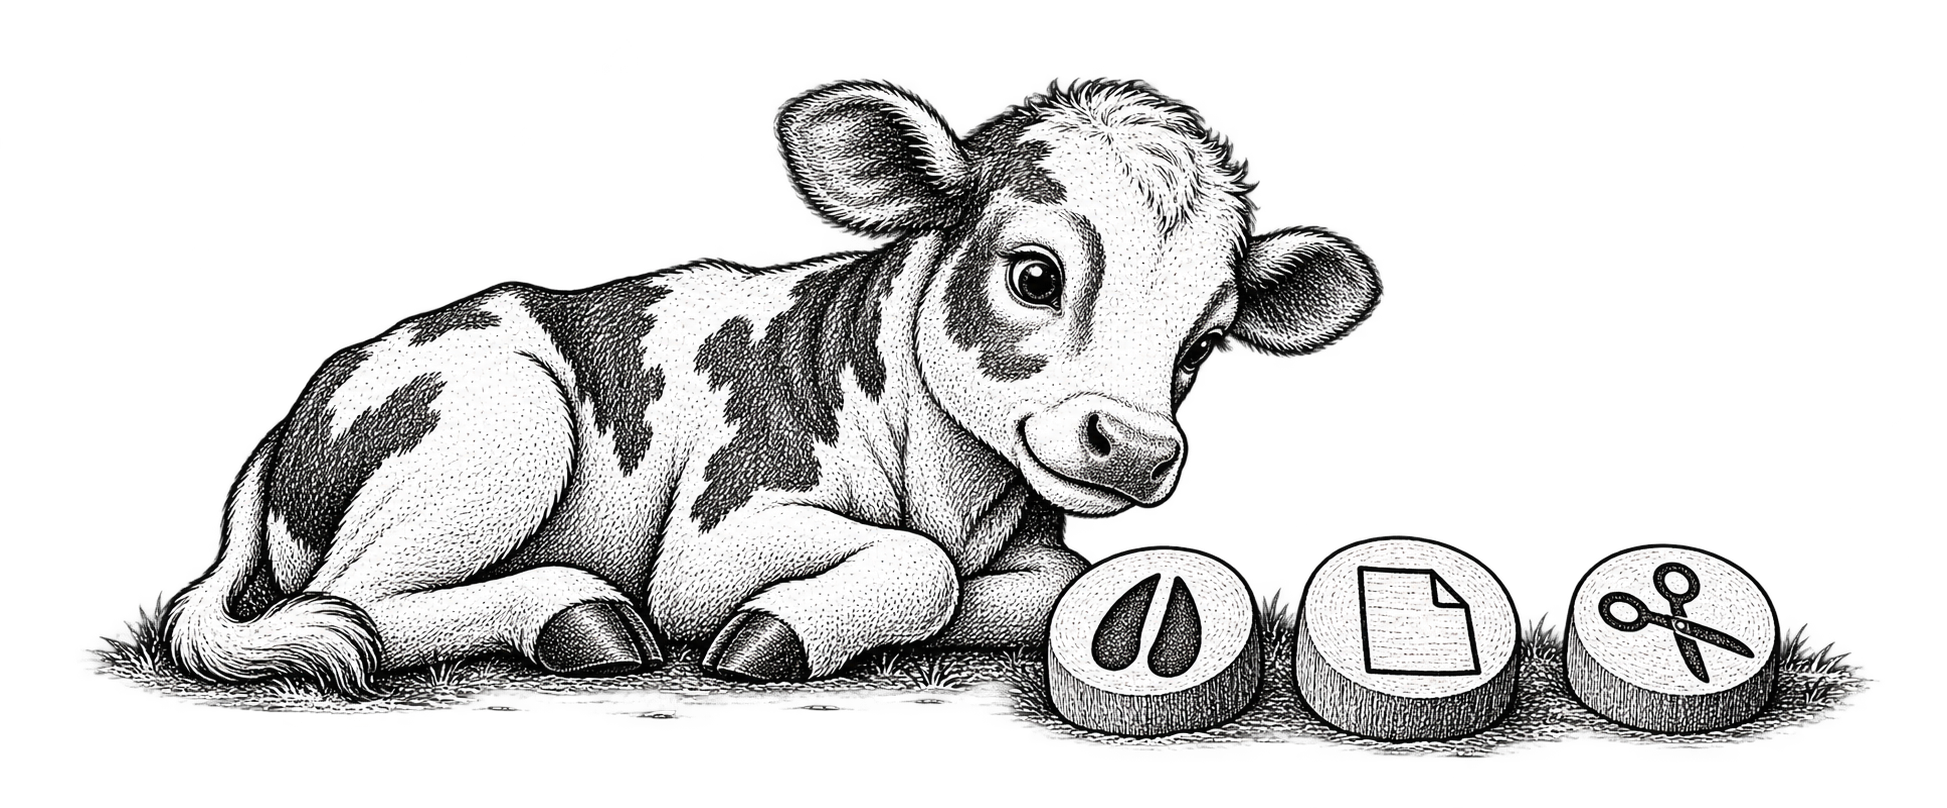
\includegraphics[width=174mm,height=94mm,keepaspectratio]{assets/cover.png}};
\node[anchor=north west,inner sep=0,text width=174mm] at ([xshift=18mm,yshift=-224mm]current page.north west)
{\fontsize{12}{16}\selectfont Questions appear in worksheet order.\\Alternative correct solutions are welcome.};
\node[anchor=west,inner sep=0] at ([xshift=18mm,yshift=-269mm]current page.north west)
{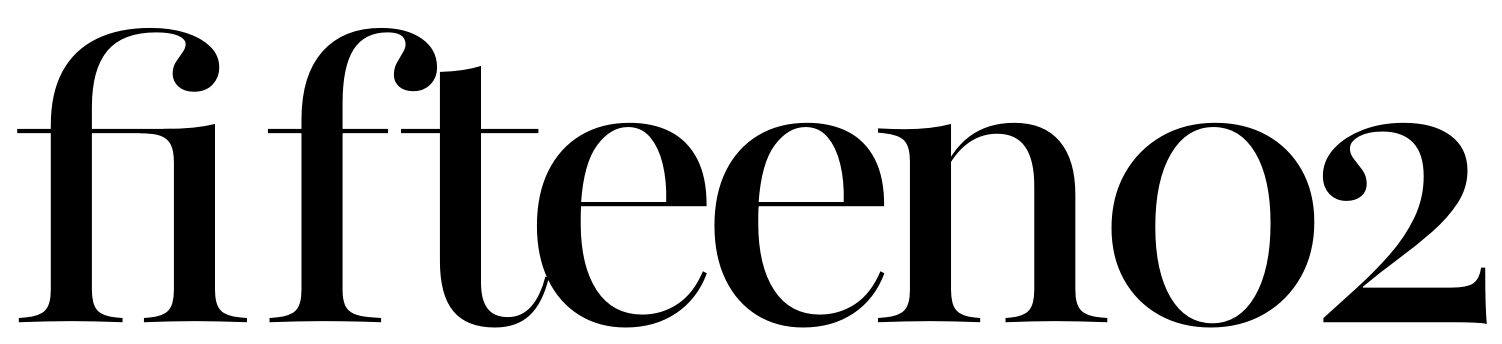
\includegraphics[width=43mm]{assets/logo.png}};
\node[anchor=east,inner sep=0] at ([xshift=192mm,yshift=-269mm]current page.north west)
{
\includegraphics[width=62mm]{assets/julians-pathfinder-monochrome.pdf}};
\end{tikzpicture}\clearpage
\topic{KEEP BESIDE YOUR WORK}{The route and the rules}
\textbf{Our route}\par Count wins when one gesture is kept throughout. Then place one change by hand. To solve longer games, record the round, switches used and ending gesture. Compare keeping that gesture with changing it, and fill a fresh table for each round.\par\medskip
\textbf{Game rules}\par John's entire sequence is known in advance. Bessie chooses H (hoof), P (paper) or S (scissors) for each round. H beats S, S beats P, and P beats H. A win scores 1; a draw or loss scores 0. Maximise Bessie's total wins.\par\medskip
\textbf{Switch rules}\par The first gesture is free. A switch is a change of gesture between two consecutive rounds. The budget, called K in the judge's statement and budget in the code, allows at most that many changes, not exactly that many. For example, H, H, P uses one switch. Number rounds from 0, so round 2 is the third round.\par\medskip
\textbf{Names used in the questions}\par \texttt{used} is the number of switches already used (written \texttt{used} in the code too). \texttt{g} is the current gesture. A score cell stores the most wins among strategies with that exact used and g after the specified round. Two different strategies may contribute to the same cell; keep the better score.\par\medskip
\textbf{Reading the tables}\par The columns headed H, P and S identify Bessie's ending gesture, not John's move. Write a dash for a state that is impossible. A score of 0 instead means a legal strategy exists but has no wins. L5-06 connects the dash to the program's negative-infinity value.\par\medskip
\textbf{Using these answers.} Each question and its supplied diagram or table appear before the answer. Completed tables, and answer diagrams where the question has one, follow the worked answer. The IDs match the worksheet; answer pages have their own page numbers. Each program is printed in full once, with imports, line numbers and a small check; a later question that uses the same program names the page where it appears and gives its own check.\par\bigskip{\color{lightink}\hrule height .4pt}\bigskip\par\markboth{Which gesture wins?}{}\begin{qblock}\begin{qblock}[0.95]
\qtopic{L5-01}{Which gesture wins?}
{\small\color{quiet}Plan gestures and count switches}\par\medskip
\textbf{Question.} H means hoof, P paper and S scissors. H beats S, S beats P, and P beats H. A win scores 1; a draw or loss scores 0. John plays H, H, S, S, P. Fill Bessie's wins in each round when she keeps H throughout, then when she keeps P or S.

\textbf{Table supplied with the question.}\par\par\medskip \begingroup\small\setlength{\tabcolsep}{4pt}\renewcommand{\arraystretch}{1.35}\begin{tabularx}{\linewidth}{>{\raggedright\arraybackslash}X>{\raggedright\arraybackslash}X>{\raggedright\arraybackslash}X>{\raggedright\arraybackslash}X>{\raggedright\arraybackslash}X>{\raggedright\arraybackslash}X}\toprule\textbf{Round} & \textbf{0} & \textbf{1} & \textbf{2} & \textbf{3} & \textbf{4}\\\midrule
John & H & H & S & S & P\\
Keep H & ? & ? & ? & ? & ?\\
Keep P & ? & ? & ? & ? & ?\\
Keep S & ? & ? & ? & ? & ?\\
\bottomrule\end{tabularx}\endgroup\par\medskip 
\par\medskip\textbf{Worked answer.} Keeping H wins twice, against the two S rounds. Keeping P wins twice, against the two H rounds. Keeping S wins once, against P. Draws and losses each contribute zero wins.

\textbf{Completed table.}\par\par\medskip \begingroup\small\setlength{\tabcolsep}{4pt}\renewcommand{\arraystretch}{1.35}\begin{tabularx}{\linewidth}{>{\raggedright\arraybackslash}X>{\raggedright\arraybackslash}X>{\raggedright\arraybackslash}X>{\raggedright\arraybackslash}X>{\raggedright\arraybackslash}X>{\raggedright\arraybackslash}X}\toprule\textbf{Round} & \textbf{0} & \textbf{1} & \textbf{2} & \textbf{3} & \textbf{4}\\\midrule
John & H & H & S & S & P\\
Keep H & 0 & 0 & 1 & 1 & 0\\
Keep P & 1 & 1 & 0 & 0 & 0\\
Keep S & 0 & 0 & 0 & 0 & 1\\
\bottomrule\end{tabularx}\endgroup\par\medskip 
\end{qblock}
\end{qblock}\par\medskip{\color{lightink}\hrule height .4pt}\bigskip
\par\markboth{Zero switches is already a useful case}{}\begin{qblock}\begin{qblock}[0.95]
\qtopic{L5-02}{Zero switches is already a useful case}
{\small\color{quiet}Plan gestures and count switches}\par\medskip
\textbf{Question.} With no switches allowed, how would you solve the whole game? What answer do you get for H, H, S, S, P?

\par\medskip\textbf{Worked answer.} Count the wins for each fixed gesture and take the largest. The answer is 2. Choosing the first gesture is free, so all three fixed strategies are available.

\end{qblock}
\end{qblock}\par\medskip{\color{lightink}\hrule height .4pt}\bigskip
\par\markboth{One well-placed switch}{}\begin{qblock}\begin{qblock}[0.95]
\qtopic{L5-03}{One well-placed switch}
{\small\color{quiet}Plan gestures and count switches}\par\medskip
\textbf{Question.} John plays H, H, S, S, P. Bessie may choose her first gesture freely and change it at most once between rounds. Find a strategy with four wins. Number rounds from 0 and identify the gap where she changes. Can one change produce five wins?

\textbf{Table supplied with the question.}\par\par\medskip \begingroup\small\setlength{\tabcolsep}{4pt}\renewcommand{\arraystretch}{1.35}\begin{tabularx}{\linewidth}{>{\raggedright\arraybackslash}X>{\raggedright\arraybackslash}X>{\raggedright\arraybackslash}X>{\raggedright\arraybackslash}X>{\raggedright\arraybackslash}X>{\raggedright\arraybackslash}X}\toprule\textbf{Round} & \textbf{0} & \textbf{1} & \textbf{2} & \textbf{3} & \textbf{4}\\\midrule
John & H & H & S & S & P\\
Bessie & ? & ? & ? & ? & ?\\
Wins & ? & ? & ? & ? & ?\\
\bottomrule\end{tabularx}\endgroup\par\medskip 
\par\medskip\textbf{Worked answer.} Play P, P, H, H, H. Switch once before round 2 and win four rounds. Winning all five would require P, P, H, H, S, which changes twice. Thus 4 is optimal.

\textbf{Completed table.}\par\par\medskip \begingroup\small\setlength{\tabcolsep}{4pt}\renewcommand{\arraystretch}{1.35}\begin{tabularx}{\linewidth}{>{\raggedright\arraybackslash}X>{\raggedright\arraybackslash}X>{\raggedright\arraybackslash}X>{\raggedright\arraybackslash}X>{\raggedright\arraybackslash}X>{\raggedright\arraybackslash}X}\toprule\textbf{Round} & \textbf{0} & \textbf{1} & \textbf{2} & \textbf{3} & \textbf{4}\\\midrule
John & H & H & S & S & P\\
Bessie & P & P & H & H & H\\
Wins & 1 & 1 & 1 & 1 & 0\\
\bottomrule\end{tabularx}\endgroup\par\medskip 
\end{qblock}
\end{qblock}\par\medskip{\color{lightink}\hrule height .4pt}\bigskip
\par\markboth{What must the state remember?}{}\begin{qblock}\begin{qblock}[0.95]
\qtopic{L5-04}{What must the state remember?}
{\small\color{quiet}Plan gestures and count switches}\par\medskip
\textbf{Question.} Two strategies have processed the same rounds and used one switch, but one ends with H and the other with P. Can their best win counts be merged into one number?

\par\medskip\textbf{Worked answer.} No. Their current gestures differ, so the next gesture may require a switch in one history but not the other. Record the processed round, switches used and current gesture.

Suppose the next selected gesture is H. A history already ending with H spends no switch; a history ending with P spends one. Therefore even equal scores and equal usage are not enough to merge those two histories.

\end{qblock}
\end{qblock}\par\medskip{\color{lightink}\hrule height .4pt}\bigskip
\par\markboth{Recursive choices with a budget}{}\begin{qblock}\begin{qblock}[0.95]
\qtopic{L5-05}{Recursive choices with a budget}
{\small\color{quiet}Store scores and compare continuations}\par\medskip
\textbf{Question.} Write hps\_cached(john, budget) using recursion. Its helper knows the next round, switches left and previous gesture. How do you handle the first round without charging a switch?

\par\smallskip{\small\textbf{Start with:}}\par\smallskip\noindent\colorbox{codepaper}{\parbox{\dimexpr\linewidth-2\fboxsep\relax}{\small\ttfamily\raggedright def hps\_cached(john, budget):\\\hspace*{2.4em}def best(i, left, previous):\\\hspace*{4.8em}return None  \# Your helper goes here.\\\hspace*{2.4em}return best(0, budget, '')}}\par
{\small\textbf{What each function returns.}\par hps\_cached(john, budget): the most rounds Bessie can win within the switch budget.\par best(i, left, previous): the most further wins from round i, with left switches available and previous as the last gesture.\par }
{\small\textbf{Hints.}}\begin{itemize}\item What does best return when no rounds remain?\item When does choosing a gesture cost a switch, and when is it free?\item Which choices are not allowed with the switches left?\end{itemize}
\par\medskip\textbf{Worked answer.} Try each gesture. Charge one switch only if a previous gesture exists and the new one differs. Reject choices that exceed the remaining budget. Add this round's win to the best continuation.

\end{qblock}
\begin{qblock}[0.95]
\medskip\textbf{One complete Python implementation: hps\_cached.}\label{ans-hps_cached}\par
\begin{lstlisting}[style=numbered]
from functools import lru_cache

BEATS = {'H': 'S', 'P': 'H', 'S': 'P'}

def hps_cached(john, budget):
    @lru_cache(None)
    def best(i, left, previous):
        if i == len(john):
            return 0
        answer = 0
        for gesture in 'HPS':
            change = int(previous != '' and gesture != previous)
            if change <= left:
                win = int(BEATS[gesture] == john[i])
                answer = max(answer, win + best(i + 1, left - change, gesture))
        return answer
    return best(0, budget, '')
\end{lstlisting}
\textbf{Check.} Run this after the function above.
\begin{lstlisting}
print(hps_cached('HHSSP', 1))
\end{lstlisting}
\textbf{Expected output.}
\begin{lstlisting}[language={}]
4
\end{lstlisting}
\textbf{Recursion depth.} Python stops recursion at about 1,000 nested calls by default, so this recursive version is for small inputs and the small and edge test files only. Use the iterative version for the medium and large files.

\end{qblock}
\end{qblock}\par\medskip{\color{lightink}\hrule height .4pt}\bigskip
\par\markboth{Exactly used versus at most allowed}{}\begin{qblock}\begin{qblock}[0.95]
\qtopic{L5-06}{Exactly used versus at most allowed}
{\small\color{quiet}Store scores and compare continuations}\par\medskip
\textbf{Question.} John plays H in round 0. Fill Bessie's scores for each ending gesture H, P and S with exactly zero switches used. Can exactly one switch have been used after just this round? Write a dash for impossible states and explain why a score of 0 would mean something different.

\textbf{Table supplied with the question.}\par\par\medskip \begingroup\small\setlength{\tabcolsep}{4pt}\renewcommand{\arraystretch}{1.35}\begin{tabularx}{\linewidth}{>{\raggedright\arraybackslash}X>{\raggedright\arraybackslash}X>{\raggedright\arraybackslash}X>{\raggedright\arraybackslash}X}\toprule\textbf{Switches used} & \textbf{End H} & \textbf{End P} & \textbf{End S}\\\midrule
0 & ? & ? & ?\\
1 & ? & ? & ?\\
\bottomrule\end{tabularx}\endgroup\par\medskip 
\par\medskip\textbf{Worked answer.} For ending gestures H, P, S, the zero-switch scores are [0, 1, 0]. Exactly one switch is impossible after one round. Mark impossible states with negative infinity, not zero.

\textbf{Completed table.}\par\par\medskip \begingroup\small\setlength{\tabcolsep}{4pt}\renewcommand{\arraystretch}{1.35}\begin{tabularx}{\linewidth}{>{\raggedright\arraybackslash}X>{\raggedright\arraybackslash}X>{\raggedright\arraybackslash}X>{\raggedright\arraybackslash}X}\toprule\textbf{Switches used} & \textbf{End H} & \textbf{End P} & \textbf{End S}\\\midrule
0 & 0 & 1 & 0\\
1 & impossible & impossible & impossible\\
\bottomrule\end{tabularx}\endgroup\par\medskip 
A switch needs a gap between two rounds. After the first round there is no such gap yet. Keeping H against John's H is legal and scores 0, whereas using exactly one switch is impossible. Those are different situations.

\end{qblock}
\end{qblock}\par\medskip{\color{lightink}\hrule height .4pt}\bigskip
\par\markboth{Stay or switch before this round}{}\begin{qblock}\begin{qblock}[0.95]
\qtopic{L5-07}{Stay or switch before this round}
{\small\color{quiet}Store scores and compare continuations}\par\medskip
\textbf{Question.} After John plays H,H, scores for ending H,P,S are [0,2,0] with no switches and [1,1,1] with exactly one. John now plays S. For an ending H with exactly one switch, compare staying with H against changing from P or S. Then fill both new score rows.

\textbf{Table supplied with the question.}\par\par\medskip \begingroup\small\setlength{\tabcolsep}{4pt}\renewcommand{\arraystretch}{1.35}\begin{tabularx}{\linewidth}{>{\raggedright\arraybackslash}X>{\raggedright\arraybackslash}X>{\raggedright\arraybackslash}X>{\raggedright\arraybackslash}X}\toprule\textbf{After H,H,S} & \textbf{End H} & \textbf{End P} & \textbf{End S}\\\midrule
0 switches & ? & ? & ?\\
1 switch & ? & ? & ?\\
\bottomrule\end{tabularx}\endgroup\par\medskip 
\par\medskip\textbf{Worked answer.} Stay with H after one earlier switch: 1 + 1 = 2. Switch now from P: 2 + 1 = 3; from S: 0 + 1 = 1. Each candidate adds this round's win once. Keep 3. The complete rows are [1,2,0] for zero switches and [3,1,2] for exactly one.

\textbf{Completed table.}\par\par\medskip \begingroup\small\setlength{\tabcolsep}{4pt}\renewcommand{\arraystretch}{1.35}\begin{tabularx}{\linewidth}{>{\raggedright\arraybackslash}X>{\raggedright\arraybackslash}X>{\raggedright\arraybackslash}X>{\raggedright\arraybackslash}X}\toprule\textbf{After H,H,S} & \textbf{End H} & \textbf{End P} & \textbf{End S}\\\midrule
0 switches & 1 & 2 & 0\\
1 switch & 3 & 1 & 2\\
\bottomrule\end{tabularx}\endgroup\par\medskip 
The new zero-switch row is [1, 2, 0]. For exactly one switch: ending H gives max(1, 2, 0) + 1 = 3; ending P gives max(1, 0, 0) + 0 = 1; ending S gives max(1, 0, 2) + 0 = 2. Each maximum compares staying with the same gesture after one switch, or switching now from another gesture after zero switches.

\end{qblock}
\end{qblock}\par\medskip{\color{lightink}\hrule height .4pt}\bigskip
\par\markboth{Trace all five rounds}{}\begin{qblock}\begin{qblock}[0.95]
\qtopic{L5-08}{Trace all five rounds}
{\small\color{quiet}Store scores and compare continuations}\par\medskip
\textbf{Question.} Trace John's rounds H,H,S,S,P. In each table column, 0 or 1 is the exact number of switches used; H, P or S is Bessie's ending gesture. Fill every row from the row immediately above it. A dash means impossible. Which final entry gives the best score with at most one switch?

\textbf{Table supplied with the question.}\par\par\medskip \begingroup\small\setlength{\tabcolsep}{4pt}\renewcommand{\arraystretch}{1.35}\begin{tabularx}{\linewidth}{>{\raggedright\arraybackslash}l>{\raggedright\arraybackslash}X>{\raggedright\arraybackslash}X>{\raggedright\arraybackslash}X>{\raggedright\arraybackslash}X>{\raggedright\arraybackslash}X>{\raggedright\arraybackslash}X}\toprule\textbf{John prefix} & \textbf{0: H} & \textbf{0: P} & \textbf{0: S} & \textbf{1: H} & \textbf{1: P} & \textbf{1: S}\\\midrule
H & 0 & 1 & 0 & - & - & -\\
HH & ? & ? & ? & ? & ? & ?\\
HHS & ? & ? & ? & ? & ? & ?\\
HHSS & ? & ? & ? & ? & ? & ?\\
HHSSP & ? & ? & ? & ? & ? & ?\\
\bottomrule\end{tabularx}\endgroup\par\medskip 
\par\medskip\textbf{Worked answer.} After all five rounds, zero-switch scores are [2,2,1] and one-switch scores are [4,2,3]. The largest score across both rows is 4, ending with H after one switch.

\textbf{Completed table.}\par\par\medskip \begingroup\small\setlength{\tabcolsep}{4pt}\renewcommand{\arraystretch}{1.35}\begin{tabularx}{\linewidth}{>{\raggedright\arraybackslash}l>{\raggedright\arraybackslash}X>{\raggedright\arraybackslash}X>{\raggedright\arraybackslash}X>{\raggedright\arraybackslash}X>{\raggedright\arraybackslash}X>{\raggedright\arraybackslash}X}\toprule\textbf{John prefix} & \textbf{0: H} & \textbf{0: P} & \textbf{0: S} & \textbf{1: H} & \textbf{1: P} & \textbf{1: S}\\\midrule
H & 0 & 1 & 0 & - & - & -\\
HH & 0 & 2 & 0 & 1 & 1 & 1\\
HHS & 1 & 2 & 0 & 3 & 1 & 2\\
HHSS & 2 & 2 & 0 & 4 & 1 & 2\\
HHSSP & 2 & 2 & 1 & 4 & 2 & 3\\
\bottomrule\end{tabularx}\endgroup\par\medskip 
The table records the best score for each exact usage and ending gesture after each prefix of John's sequence. The final maximum is max(2, 2, 1, 4, 2, 3) = 4. A strategy attaining it is P, P, H, H, H.

\end{qblock}
\end{qblock}\par\medskip{\color{lightink}\hrule height .4pt}\bigskip
\par\markboth{Keep just the previous round}{}\begin{qblock}\begin{qblock}[0.95]
\qtopic{L5-09}{Keep just the previous round}
{\small\color{quiet}Store scores and compare continuations}\par\medskip
\textbf{Question.} Write hps\_table(john, budget) using a loop over rounds. Here used counts switches already used and g is the ending gesture. before[used][g] stores the best score after the previous round; now[used][g] includes the current round. Compare staying and switching. Why must now be fresh? Return the best score using at most budget switches (K in the original statement).

\par\smallskip{\small\textbf{Start with:}}\par\smallskip\noindent\colorbox{codepaper}{\parbox{\dimexpr\linewidth-2\fboxsep\relax}{\small\ttfamily\raggedright def hps\_table(john, budget):\\\hspace*{2.4em}return None  \# Replace with your answer.}}\par
{\small\textbf{What each function returns.}\par hps\_table(john, budget): the most rounds Bessie can win within the switch budget.\par }
{\small\textbf{Hints.}}\begin{itemize}\item What are the scores after round 0, and which states are impossible then?\item For a new cell, which cells of before lead to it by staying, and which by switching?\item What should an impossible state hold so that max ignores it?\end{itemize}
\par\medskip\textbf{Worked answer.} before holds completed scores for the previous round; now holds scores for the current round. Keep the old table unchanged while all new cells are calculated, so a round cannot be counted twice. For at most K switches, return the maximum over every ending gesture and every usage row from 0 to K.

For each new round, all candidate scores must come from the completed previous round. Reading a cell already updated for the current round could reuse this round's score or spend another switch in the same gap. A fresh now table keeps the two rounds separate.

\end{qblock}
\begin{qblock}[0.95]
\medskip\textbf{One complete Python implementation: hps\_table.}\label{ans-hps_table}\par
\begin{lstlisting}[style=numbered]
BEATS = {'H': 'S', 'P': 'H', 'S': 'P'}

def hps_table(john, budget):
    if not john:
        return 0
    gestures = 'HPS'
    impossible = -float('inf')
    before = [[impossible] * 3 for _ in range(budget + 1)]
    for g, gesture in enumerate(gestures):
        before[0][g] = int(BEATS[gesture] == john[0])
    for opponent in john[1:]:
        now = [[impossible] * 3 for _ in range(budget + 1)]
        for used in range(budget + 1):
            for g, gesture in enumerate(gestures):
                best_before = before[used][g]
                if used > 0:
                    for old in range(3):
                        if old != g:
                            best_before = max(best_before, before[used - 1][old])
                now[used][g] = best_before + int(BEATS[gesture] == opponent)
        before = now
    return int(max(max(row) for row in before))
\end{lstlisting}
\textbf{Check.} Run this after the function above.
\begin{lstlisting}
print(hps_table('HHSSP', 1))
\end{lstlisting}
\textbf{Expected output.}
\begin{lstlisting}[language={}]
4
\end{lstlisting}
\end{qblock}
\end{qblock}\par\medskip{\color{lightink}\hrule height .4pt}\bigskip
\par\markboth{Your turn: three different budgets}{}\begin{qblock}\begin{qblock}[0.95]
\qtopic{L5-10}{Your turn: three different budgets}
{\small\color{quiet}Test the budget and explain the state}\par\medskip
\textbf{Question.} Test your hps\_table(john, budget) from L5-09. For John = H,P,S, predict the best win count with budgets 0, 1 and 2. Give one strategy for each budget, then run your function.

\par\medskip\textbf{Worked answer.} Budget 0: 1 win, for example P,P,P. Budget 1: 2 wins, for example P,S,S. Budget 2: 3 wins with P,S,H. The first gesture is free in every case.

\end{qblock}
\end{qblock}\par\medskip{\color{lightink}\hrule height .4pt}\bigskip
\par\markboth{More switches need not help}{}\begin{qblock}\begin{qblock}[0.95]
\qtopic{L5-11}{More switches need not help}
{\small\color{quiet}Test the budget and explain the state}\par\medskip
\textbf{Question.} Test your hps\_table(john, budget) from L5-09 on John = H,H,H with budgets 0 and 2, and on one round against S with budget 0. Predict each answer before running it. What should happen when the budget exceeds the useful number of changes?

\par\medskip\textbf{Worked answer.} For H,H,H, both budgets give 3 wins by keeping P. For one S round the answer is 1 by choosing H, with no switch needed. Extra budget never forces extra changes.

\end{qblock}
\end{qblock}\par\medskip{\color{lightink}\hrule height .4pt}\bigskip
\par\markboth{The state is the explanation}{}\begin{qblock}\begin{qblock}[0.95]
\qtopic{L5-12}{The state is the explanation}
{\small\color{quiet}Test the budget and explain the state}\par\medskip
\textbf{Question.} Choose a cell from the five-round score table and explain its round, exact switch count, ending gesture and stored score. Why can we forget the earlier gesture sequence once these facts and its best score are known? Compare this with Tower or Array Description.

\textbf{Table supplied with the question.}\par\par\medskip \begingroup\small\setlength{\tabcolsep}{4pt}\renewcommand{\arraystretch}{1.35}\begin{tabularx}{\linewidth}{>{\raggedright\arraybackslash}X>{\raggedright\arraybackslash}X>{\raggedright\arraybackslash}X>{\raggedright\arraybackslash}X}\toprule\textbf{John prefix} & \textbf{Switches used} & \textbf{Ending gesture} & \textbf{Stored score}\\\midrule
 &  &  & \\
\bottomrule\end{tabularx}\endgroup\par\medskip 
\par\medskip\textbf{Worked answer.} After H,H,S, the cell for exactly one switch and ending H stores 3: P,P,H wins every round. A worse strategy at that same round, usage and gesture cannot improve future choices: it has the same remaining moves but fewer wins. Tower similarly keeps position and next player; Array Description keeps position and previous value.

\textbf{Completed table.}\par\par\medskip \begingroup\small\setlength{\tabcolsep}{4pt}\renewcommand{\arraystretch}{1.35}\begin{tabularx}{\linewidth}{>{\raggedright\arraybackslash}X>{\raggedright\arraybackslash}X>{\raggedright\arraybackslash}X>{\raggedright\arraybackslash}X}\toprule\textbf{John prefix} & \textbf{Switches used} & \textbf{Ending gesture} & \textbf{Stored score}\\\midrule
HHS & 1 & H & 3\\
\bottomrule\end{tabularx}\endgroup\par\medskip 
\end{qblock}
\end{qblock}\par\medskip{\color{lightink}\hrule height .4pt}\bigskip
\end{document}